% Options for packages loaded elsewhere
\PassOptionsToPackage{unicode}{hyperref}
\PassOptionsToPackage{hyphens}{url}
\PassOptionsToPackage{dvipsnames,svgnames,x11names}{xcolor}
%
\documentclass[
  letterpaper,
  DIV=11,
  numbers=noendperiod]{scrartcl}

\usepackage{amsmath,amssymb}
\usepackage{iftex}
\ifPDFTeX
  \usepackage[T1]{fontenc}
  \usepackage[utf8]{inputenc}
  \usepackage{textcomp} % provide euro and other symbols
\else % if luatex or xetex
  \usepackage{unicode-math}
  \defaultfontfeatures{Scale=MatchLowercase}
  \defaultfontfeatures[\rmfamily]{Ligatures=TeX,Scale=1}
\fi
\usepackage{lmodern}
\ifPDFTeX\else  
    % xetex/luatex font selection
\fi
% Use upquote if available, for straight quotes in verbatim environments
\IfFileExists{upquote.sty}{\usepackage{upquote}}{}
\IfFileExists{microtype.sty}{% use microtype if available
  \usepackage[]{microtype}
  \UseMicrotypeSet[protrusion]{basicmath} % disable protrusion for tt fonts
}{}
\makeatletter
\@ifundefined{KOMAClassName}{% if non-KOMA class
  \IfFileExists{parskip.sty}{%
    \usepackage{parskip}
  }{% else
    \setlength{\parindent}{0pt}
    \setlength{\parskip}{6pt plus 2pt minus 1pt}}
}{% if KOMA class
  \KOMAoptions{parskip=half}}
\makeatother
\usepackage{xcolor}
\setlength{\emergencystretch}{3em} % prevent overfull lines
\setcounter{secnumdepth}{-\maxdimen} % remove section numbering
% Make \paragraph and \subparagraph free-standing
\ifx\paragraph\undefined\else
  \let\oldparagraph\paragraph
  \renewcommand{\paragraph}[1]{\oldparagraph{#1}\mbox{}}
\fi
\ifx\subparagraph\undefined\else
  \let\oldsubparagraph\subparagraph
  \renewcommand{\subparagraph}[1]{\oldsubparagraph{#1}\mbox{}}
\fi

\usepackage{color}
\usepackage{fancyvrb}
\newcommand{\VerbBar}{|}
\newcommand{\VERB}{\Verb[commandchars=\\\{\}]}
\DefineVerbatimEnvironment{Highlighting}{Verbatim}{commandchars=\\\{\}}
% Add ',fontsize=\small' for more characters per line
\usepackage{framed}
\definecolor{shadecolor}{RGB}{241,243,245}
\newenvironment{Shaded}{\begin{snugshade}}{\end{snugshade}}
\newcommand{\AlertTok}[1]{\textcolor[rgb]{0.68,0.00,0.00}{#1}}
\newcommand{\AnnotationTok}[1]{\textcolor[rgb]{0.37,0.37,0.37}{#1}}
\newcommand{\AttributeTok}[1]{\textcolor[rgb]{0.40,0.45,0.13}{#1}}
\newcommand{\BaseNTok}[1]{\textcolor[rgb]{0.68,0.00,0.00}{#1}}
\newcommand{\BuiltInTok}[1]{\textcolor[rgb]{0.00,0.23,0.31}{#1}}
\newcommand{\CharTok}[1]{\textcolor[rgb]{0.13,0.47,0.30}{#1}}
\newcommand{\CommentTok}[1]{\textcolor[rgb]{0.37,0.37,0.37}{#1}}
\newcommand{\CommentVarTok}[1]{\textcolor[rgb]{0.37,0.37,0.37}{\textit{#1}}}
\newcommand{\ConstantTok}[1]{\textcolor[rgb]{0.56,0.35,0.01}{#1}}
\newcommand{\ControlFlowTok}[1]{\textcolor[rgb]{0.00,0.23,0.31}{#1}}
\newcommand{\DataTypeTok}[1]{\textcolor[rgb]{0.68,0.00,0.00}{#1}}
\newcommand{\DecValTok}[1]{\textcolor[rgb]{0.68,0.00,0.00}{#1}}
\newcommand{\DocumentationTok}[1]{\textcolor[rgb]{0.37,0.37,0.37}{\textit{#1}}}
\newcommand{\ErrorTok}[1]{\textcolor[rgb]{0.68,0.00,0.00}{#1}}
\newcommand{\ExtensionTok}[1]{\textcolor[rgb]{0.00,0.23,0.31}{#1}}
\newcommand{\FloatTok}[1]{\textcolor[rgb]{0.68,0.00,0.00}{#1}}
\newcommand{\FunctionTok}[1]{\textcolor[rgb]{0.28,0.35,0.67}{#1}}
\newcommand{\ImportTok}[1]{\textcolor[rgb]{0.00,0.46,0.62}{#1}}
\newcommand{\InformationTok}[1]{\textcolor[rgb]{0.37,0.37,0.37}{#1}}
\newcommand{\KeywordTok}[1]{\textcolor[rgb]{0.00,0.23,0.31}{#1}}
\newcommand{\NormalTok}[1]{\textcolor[rgb]{0.00,0.23,0.31}{#1}}
\newcommand{\OperatorTok}[1]{\textcolor[rgb]{0.37,0.37,0.37}{#1}}
\newcommand{\OtherTok}[1]{\textcolor[rgb]{0.00,0.23,0.31}{#1}}
\newcommand{\PreprocessorTok}[1]{\textcolor[rgb]{0.68,0.00,0.00}{#1}}
\newcommand{\RegionMarkerTok}[1]{\textcolor[rgb]{0.00,0.23,0.31}{#1}}
\newcommand{\SpecialCharTok}[1]{\textcolor[rgb]{0.37,0.37,0.37}{#1}}
\newcommand{\SpecialStringTok}[1]{\textcolor[rgb]{0.13,0.47,0.30}{#1}}
\newcommand{\StringTok}[1]{\textcolor[rgb]{0.13,0.47,0.30}{#1}}
\newcommand{\VariableTok}[1]{\textcolor[rgb]{0.07,0.07,0.07}{#1}}
\newcommand{\VerbatimStringTok}[1]{\textcolor[rgb]{0.13,0.47,0.30}{#1}}
\newcommand{\WarningTok}[1]{\textcolor[rgb]{0.37,0.37,0.37}{\textit{#1}}}

\providecommand{\tightlist}{%
  \setlength{\itemsep}{0pt}\setlength{\parskip}{0pt}}\usepackage{longtable,booktabs,array}
\usepackage{calc} % for calculating minipage widths
% Correct order of tables after \paragraph or \subparagraph
\usepackage{etoolbox}
\makeatletter
\patchcmd\longtable{\par}{\if@noskipsec\mbox{}\fi\par}{}{}
\makeatother
% Allow footnotes in longtable head/foot
\IfFileExists{footnotehyper.sty}{\usepackage{footnotehyper}}{\usepackage{footnote}}
\makesavenoteenv{longtable}
\usepackage{graphicx}
\makeatletter
\def\maxwidth{\ifdim\Gin@nat@width>\linewidth\linewidth\else\Gin@nat@width\fi}
\def\maxheight{\ifdim\Gin@nat@height>\textheight\textheight\else\Gin@nat@height\fi}
\makeatother
% Scale images if necessary, so that they will not overflow the page
% margins by default, and it is still possible to overwrite the defaults
% using explicit options in \includegraphics[width, height, ...]{}
\setkeys{Gin}{width=\maxwidth,height=\maxheight,keepaspectratio}
% Set default figure placement to htbp
\makeatletter
\def\fps@figure{htbp}
\makeatother

\KOMAoption{captions}{tableheading}
\makeatletter
\makeatother
\makeatletter
\makeatother
\makeatletter
\@ifpackageloaded{caption}{}{\usepackage{caption}}
\AtBeginDocument{%
\ifdefined\contentsname
  \renewcommand*\contentsname{Table of contents}
\else
  \newcommand\contentsname{Table of contents}
\fi
\ifdefined\listfigurename
  \renewcommand*\listfigurename{List of Figures}
\else
  \newcommand\listfigurename{List of Figures}
\fi
\ifdefined\listtablename
  \renewcommand*\listtablename{List of Tables}
\else
  \newcommand\listtablename{List of Tables}
\fi
\ifdefined\figurename
  \renewcommand*\figurename{Figure}
\else
  \newcommand\figurename{Figure}
\fi
\ifdefined\tablename
  \renewcommand*\tablename{Table}
\else
  \newcommand\tablename{Table}
\fi
}
\@ifpackageloaded{float}{}{\usepackage{float}}
\floatstyle{ruled}
\@ifundefined{c@chapter}{\newfloat{codelisting}{h}{lop}}{\newfloat{codelisting}{h}{lop}[chapter]}
\floatname{codelisting}{Listing}
\newcommand*\listoflistings{\listof{codelisting}{List of Listings}}
\makeatother
\makeatletter
\@ifpackageloaded{caption}{}{\usepackage{caption}}
\@ifpackageloaded{subcaption}{}{\usepackage{subcaption}}
\makeatother
\makeatletter
\@ifpackageloaded{tcolorbox}{}{\usepackage[skins,breakable]{tcolorbox}}
\makeatother
\makeatletter
\@ifundefined{shadecolor}{\definecolor{shadecolor}{rgb}{.97, .97, .97}}
\makeatother
\makeatletter
\makeatother
\makeatletter
\makeatother
\ifLuaTeX
  \usepackage{selnolig}  % disable illegal ligatures
\fi
\IfFileExists{bookmark.sty}{\usepackage{bookmark}}{\usepackage{hyperref}}
\IfFileExists{xurl.sty}{\usepackage{xurl}}{} % add URL line breaks if available
\urlstyle{same} % disable monospaced font for URLs
\hypersetup{
  pdftitle={Entrega1},
  colorlinks=true,
  linkcolor={blue},
  filecolor={Maroon},
  citecolor={Blue},
  urlcolor={Blue},
  pdfcreator={LaTeX via pandoc}}

\title{Entrega1}
\author{}
\date{}

\begin{document}
\maketitle
\ifdefined\Shaded\renewenvironment{Shaded}{\begin{tcolorbox}[breakable, enhanced, boxrule=0pt, interior hidden, borderline west={3pt}{0pt}{shadecolor}, sharp corners, frame hidden]}{\end{tcolorbox}}\fi

\href{https://github.com/GSMir/Entrega1.git}{Repositorio}

\hypertarget{cargamos-las-liberuxedas-necesarias}{%
\subsection{Cargamos las liberías
necesarias}\label{cargamos-las-liberuxedas-necesarias}}

\begin{Shaded}
\begin{Highlighting}[]
\CommentTok{\#install.packages("palmerpenguins",dep=TRUE)}
\FunctionTok{library}\NormalTok{(}\StringTok{"palmerpenguins"}\NormalTok{)}
\FunctionTok{print}\NormalTok{(penguins, }\AttributeTok{width =} \DecValTok{50}\NormalTok{)}
\end{Highlighting}
\end{Shaded}

\begin{verbatim}
# A tibble: 344 x 8
   species island    bill_length_mm bill_depth_mm
   <fct>   <fct>              <dbl>         <dbl>
 1 Adelie  Torgersen           39.1          18.7
 2 Adelie  Torgersen           39.5          17.4
 3 Adelie  Torgersen           40.3          18  
 4 Adelie  Torgersen           NA            NA  
 5 Adelie  Torgersen           36.7          19.3
 6 Adelie  Torgersen           39.3          20.6
 7 Adelie  Torgersen           38.9          17.8
 8 Adelie  Torgersen           39.2          19.6
 9 Adelie  Torgersen           34.1          18.1
10 Adelie  Torgersen           42            20.2
# i 334 more rows
# i 4 more variables: flipper_length_mm <int>,
#   body_mass_g <int>, sex <fct>, year <int>
\end{verbatim}

Hay 344 observaciones de pingüinos, y 8 variables diferentes.

\hypertarget{vamos-a-mirar-cada-una-de-las-variables}{%
\subsection{Vamos a mirar cada una de las
variables:}\label{vamos-a-mirar-cada-una-de-las-variables}}

\begin{Shaded}
\begin{Highlighting}[]
\FunctionTok{summary}\NormalTok{(penguins)}
\end{Highlighting}
\end{Shaded}

\begin{verbatim}
      species          island    bill_length_mm  bill_depth_mm  
 Adelie   :152   Biscoe   :168   Min.   :32.10   Min.   :13.10  
 Chinstrap: 68   Dream    :124   1st Qu.:39.23   1st Qu.:15.60  
 Gentoo   :124   Torgersen: 52   Median :44.45   Median :17.30  
                                 Mean   :43.92   Mean   :17.15  
                                 3rd Qu.:48.50   3rd Qu.:18.70  
                                 Max.   :59.60   Max.   :21.50  
                                 NA's   :2       NA's   :2      
 flipper_length_mm  body_mass_g       sex           year     
 Min.   :172.0     Min.   :2700   female:165   Min.   :2007  
 1st Qu.:190.0     1st Qu.:3550   male  :168   1st Qu.:2007  
 Median :197.0     Median :4050   NA's  : 11   Median :2008  
 Mean   :200.9     Mean   :4202                Mean   :2008  
 3rd Qu.:213.0     3rd Qu.:4750                3rd Qu.:2009  
 Max.   :231.0     Max.   :6300                Max.   :2009  
 NA's   :2         NA's   :2                                 
\end{verbatim}

\hypertarget{species}{%
\subsubsection{Species}\label{species}}

\begin{Shaded}
\begin{Highlighting}[]
\FunctionTok{class}\NormalTok{(penguins}\SpecialCharTok{$}\NormalTok{species)}
\end{Highlighting}
\end{Shaded}

\begin{verbatim}
[1] "factor"
\end{verbatim}

Podemos observar que hay 3 espécies diferentes, ``Adelie'',
``Chinstrap'' y ``Gentoo''. Es una variable del tipo ``factor''.

\hypertarget{island}{%
\subsubsection{Island}\label{island}}

\begin{Shaded}
\begin{Highlighting}[]
\FunctionTok{class}\NormalTok{(penguins}\SpecialCharTok{$}\NormalTok{island)}
\end{Highlighting}
\end{Shaded}

\begin{verbatim}
[1] "factor"
\end{verbatim}

Podemos observar que hay 3 islas diferentes, ``Biscoe'', ``Dream'' y
``Torgersen''. Es una variable del tipo ``factor''.

\hypertarget{bill_length_mm}{%
\subsubsection{Bill\_length\_mm}\label{bill_length_mm}}

\begin{Shaded}
\begin{Highlighting}[]
\FunctionTok{class}\NormalTok{(penguins}\SpecialCharTok{$}\NormalTok{bill\_length\_mm)}
\end{Highlighting}
\end{Shaded}

\begin{verbatim}
[1] "numeric"
\end{verbatim}

Hace referéncia a la longitud del pico de los pingüinos, en mm. Es una
variable del tipo ``numeric''. Van en un rango de 32.1mm a 59.6mm. Con
una media de 43.92mm

\hypertarget{bill_depth_mm}{%
\subsubsection{Bill\_depth\_mm}\label{bill_depth_mm}}

\begin{Shaded}
\begin{Highlighting}[]
\FunctionTok{class}\NormalTok{(penguins}\SpecialCharTok{$}\NormalTok{bill\_depth\_mm)}
\end{Highlighting}
\end{Shaded}

\begin{verbatim}
[1] "numeric"
\end{verbatim}

Hace referéncia a la amplitud del pico de los pingüinos, en mm. Es una
variable del tipo ``numeric''. Van en un rango de 13.1mm a 21.5mm. Con
una media de 17.15mm.

\hypertarget{flipper_length_mm}{%
\subsubsection{Flipper\_length\_mm}\label{flipper_length_mm}}

\begin{Shaded}
\begin{Highlighting}[]
\FunctionTok{class}\NormalTok{(penguins}\SpecialCharTok{$}\NormalTok{flipper\_length\_mm)}
\end{Highlighting}
\end{Shaded}

\begin{verbatim}
[1] "integer"
\end{verbatim}

Hace referéncia a la longitud de las aletas de los pingüinos, en mm. Es
una variable del tipo ``integer''. Van en un rango de 172.0mm a 231.0mm.
Con una media de 200.9mm.

\hypertarget{body_mass_g}{%
\subsubsection{Body\_mass\_g}\label{body_mass_g}}

\begin{Shaded}
\begin{Highlighting}[]
\FunctionTok{class}\NormalTok{(penguins}\SpecialCharTok{$}\NormalTok{body\_mass\_g)}
\end{Highlighting}
\end{Shaded}

\begin{verbatim}
[1] "integer"
\end{verbatim}

Hace referéncia a la masa de los pingüinos, en g. Es una variable del
tipo ``integer''. Van en un rango de 2700g a 6300g. Con una media de
4202g.

\hypertarget{sex}{%
\subsubsection{Sex}\label{sex}}

\begin{Shaded}
\begin{Highlighting}[]
\FunctionTok{class}\NormalTok{(penguins}\SpecialCharTok{$}\NormalTok{sex)}
\end{Highlighting}
\end{Shaded}

\begin{verbatim}
[1] "factor"
\end{verbatim}

Hace referéncia al sexo cromosómico de los pingüinos. Es una variable de
tipo ``factor'', con los valores de Macho y Hembra.

\hypertarget{year}{%
\subsubsection{Year}\label{year}}

\begin{Shaded}
\begin{Highlighting}[]
\FunctionTok{class}\NormalTok{(penguins}\SpecialCharTok{$}\NormalTok{year)}
\end{Highlighting}
\end{Shaded}

\begin{verbatim}
[1] "integer"
\end{verbatim}

Hace referéncia al año de nacimiento de los pingüinos. Va del año 2007
al 2009. Es una variable de tipo ``integer''; para trabajar mejor con
esta variable la vamos a pasar a tipo ``factor''.

\begin{Shaded}
\begin{Highlighting}[]
\NormalTok{penguins}\SpecialCharTok{$}\NormalTok{year }\OtherTok{=} \FunctionTok{as.factor}\NormalTok{(penguins}\SpecialCharTok{$}\NormalTok{year)}
\end{Highlighting}
\end{Shaded}

\hypertarget{estudio-inferencial}{%
\subsection{Estudio inferencial}\label{estudio-inferencial}}

\hypertarget{media-de-la-longitud-de-los-picos}{%
\subsubsection{Media de la longitud de los
picos}\label{media-de-la-longitud-de-los-picos}}

Vamos a hacer un boxplot para comprobar si hay diferencias
significativas entre las medias de las longitudes de los picos en
referencia a las especies de pingüinos.

\begin{Shaded}
\begin{Highlighting}[]
\FunctionTok{boxplot}\NormalTok{(penguins}\SpecialCharTok{$}\NormalTok{bill\_length\_mm}\SpecialCharTok{\textasciitilde{}}\NormalTok{penguins}\SpecialCharTok{$}\NormalTok{species,}\AttributeTok{ylab =} \StringTok{"Longitud del pico"}\NormalTok{,}\AttributeTok{xlab =} \StringTok{"Especies"}\NormalTok{)}
\end{Highlighting}
\end{Shaded}

\begin{figure}[H]

{\centering 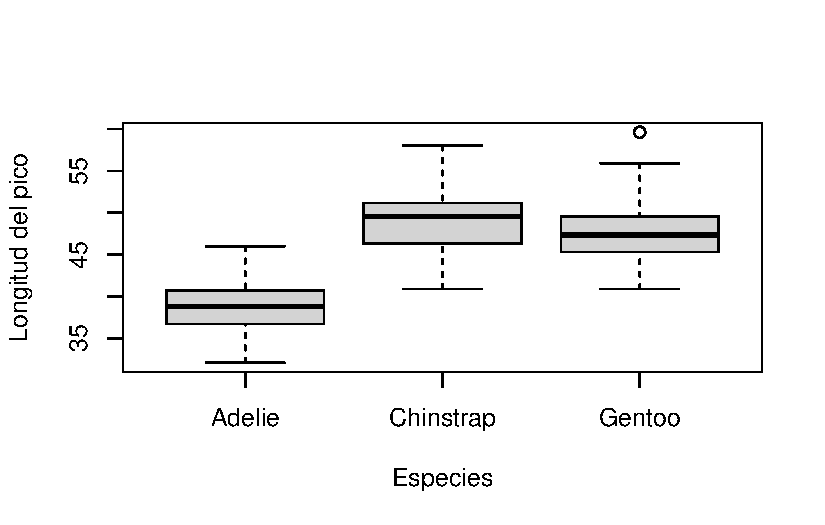
\includegraphics{Entrega1_files/figure-pdf/unnamed-chunk-24-1.pdf}

}

\end{figure}

Observamos que la mediana de Adelie es bastante más pequeña que el
resto, vamos a comprobarlo mediante un t.test.

\begin{Shaded}
\begin{Highlighting}[]
\FunctionTok{t.test}\NormalTok{(penguins}\SpecialCharTok{$}\NormalTok{bill\_length\_mm[penguins}\SpecialCharTok{$}\NormalTok{species}\SpecialCharTok{==}\StringTok{"Adelie"}\NormalTok{],penguins}\SpecialCharTok{$}\NormalTok{bill\_length\_mm[penguins}\SpecialCharTok{$}\NormalTok{species}\SpecialCharTok{==}\StringTok{"Gentoo"}\NormalTok{],}\AttributeTok{conf.level =} \FloatTok{0.95}\NormalTok{,}\AttributeTok{alternative =} \StringTok{"less"}\NormalTok{,}\AttributeTok{paired =} \ConstantTok{FALSE}\NormalTok{,}\AttributeTok{var.equal =} \ConstantTok{FALSE}\NormalTok{)}
\end{Highlighting}
\end{Shaded}

\begin{verbatim}

    Welch Two Sample t-test

data:  penguins$bill_length_mm[penguins$species == "Adelie"] and penguins$bill_length_mm[penguins$species == "Gentoo"]
t = -24.725, df = 242.58, p-value < 2.2e-16
alternative hypothesis: true difference in means is less than 0
95 percent confidence interval:
      -Inf -8.131593
sample estimates:
mean of x mean of y 
 38.79139  47.50488 
\end{verbatim}

\begin{Shaded}
\begin{Highlighting}[]
\FunctionTok{t.test}\NormalTok{(penguins}\SpecialCharTok{$}\NormalTok{bill\_length\_mm[penguins}\SpecialCharTok{$}\NormalTok{species}\SpecialCharTok{==}\StringTok{"Adelie"}\NormalTok{],penguins}\SpecialCharTok{$}\NormalTok{bill\_length\_mm[penguins}\SpecialCharTok{$}\NormalTok{species}\SpecialCharTok{==}\StringTok{"Chinstrap"}\NormalTok{],}\AttributeTok{conf.level =} \FloatTok{0.95}\NormalTok{,}\AttributeTok{alternative =} \StringTok{"less"}\NormalTok{,}\AttributeTok{paired =} \ConstantTok{FALSE}\NormalTok{,}\AttributeTok{var.equal =} \ConstantTok{FALSE}\NormalTok{)}
\end{Highlighting}
\end{Shaded}

\begin{verbatim}

    Welch Two Sample t-test

data:  penguins$bill_length_mm[penguins$species == "Adelie"] and penguins$bill_length_mm[penguins$species == "Chinstrap"]
t = -21.865, df = 106.97, p-value < 2.2e-16
alternative hypothesis: true difference in means is less than 0
95 percent confidence interval:
      -Inf -9.280348
sample estimates:
mean of x mean of y 
 38.79139  48.83382 
\end{verbatim}

Podemos observar que los dos t.test nos sale un p-valor mas pequeño que
0.05, por lo tanto podemos afirmar la hipótesis inicial; la media de
longitud de los picos de la especia ``Adelie'' es más pequeña que la de
las otras dos.

Ahora vamos a observar si hay diferencias significativas de la longitud
del pico entre una misma especie y las islas donde habitan. Primero
vamos a comprobar en que islas viven las diferentes especies de
pingüinos.

\begin{Shaded}
\begin{Highlighting}[]
\FunctionTok{table}\NormalTok{(penguins}\SpecialCharTok{$}\NormalTok{island[penguins}\SpecialCharTok{$}\NormalTok{species}\SpecialCharTok{==}\StringTok{"Adelie"}\NormalTok{])}
\end{Highlighting}
\end{Shaded}

\begin{verbatim}

   Biscoe     Dream Torgersen 
       44        56        52 
\end{verbatim}

\begin{Shaded}
\begin{Highlighting}[]
\FunctionTok{table}\NormalTok{(penguins}\SpecialCharTok{$}\NormalTok{island[penguins}\SpecialCharTok{$}\NormalTok{species}\SpecialCharTok{==}\StringTok{"Gentoo"}\NormalTok{])}
\end{Highlighting}
\end{Shaded}

\begin{verbatim}

   Biscoe     Dream Torgersen 
      124         0         0 
\end{verbatim}

\begin{Shaded}
\begin{Highlighting}[]
\FunctionTok{table}\NormalTok{(penguins}\SpecialCharTok{$}\NormalTok{island[penguins}\SpecialCharTok{$}\NormalTok{species}\SpecialCharTok{==}\StringTok{"Chinstrap"}\NormalTok{])}
\end{Highlighting}
\end{Shaded}

\begin{verbatim}

   Biscoe     Dream Torgersen 
        0        68         0 
\end{verbatim}

Observamos que la única especie que habita en más de una isla es la
``Adelie'', por lo tanto realizamos un boxplot de las longitudes del
pico centrándonos en esa especie y las islas donde habitan.

\begin{Shaded}
\begin{Highlighting}[]
\FunctionTok{boxplot}\NormalTok{(penguins}\SpecialCharTok{$}\NormalTok{bill\_length\_mm[penguins}\SpecialCharTok{$}\NormalTok{species}\SpecialCharTok{==}\StringTok{"Adelie"}\NormalTok{]}\SpecialCharTok{\textasciitilde{}}\NormalTok{penguins}\SpecialCharTok{$}\NormalTok{island[penguins}\SpecialCharTok{$}\NormalTok{species}\SpecialCharTok{==}\StringTok{"Adelie"}\NormalTok{],}\AttributeTok{ylab =} \StringTok{"Longitud del pico de Adelie"}\NormalTok{,}\AttributeTok{xlab =} \StringTok{"Islas"}\NormalTok{)}
\end{Highlighting}
\end{Shaded}

\begin{figure}[H]

{\centering 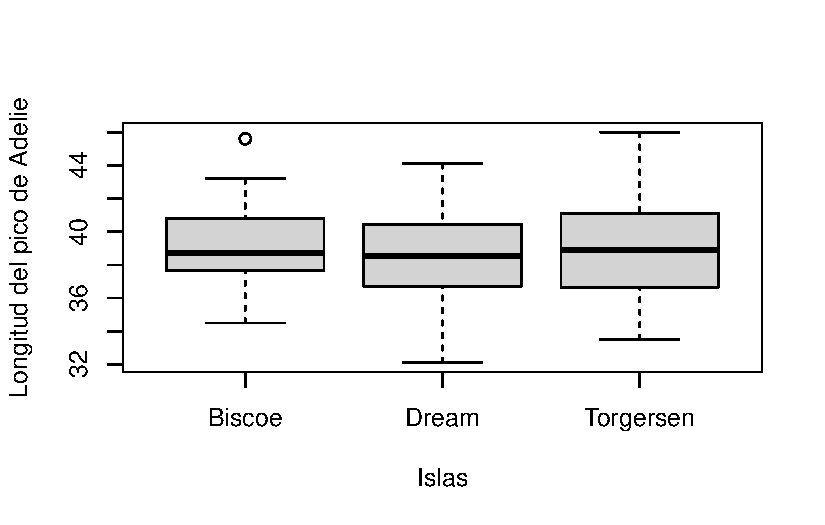
\includegraphics{Entrega1_files/figure-pdf/unnamed-chunk-30-1.pdf}

}

\end{figure}

No podemos obervar diferencias significativas.

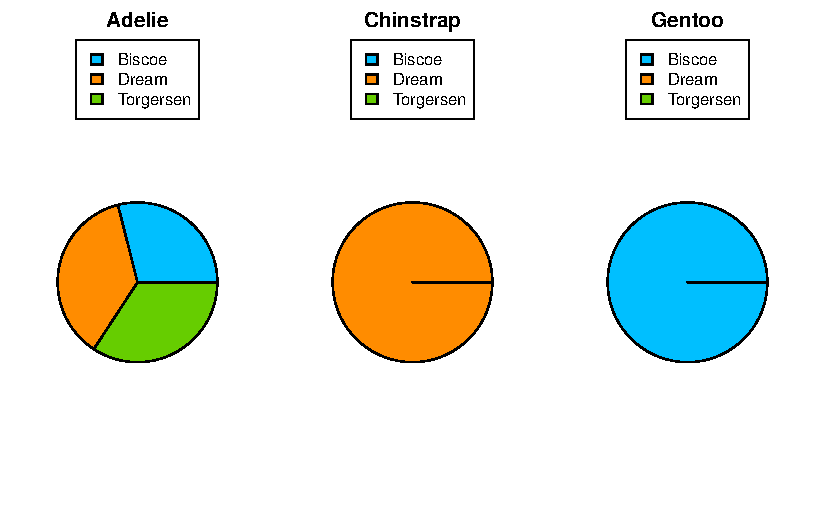
\includegraphics{Entrega1_files/figure-pdf/unnamed-chunk-32-1.pdf}



\end{document}
